\chapter{Introduction}

\epigraph{I don't like discussing cricket off the field.}{MS Dhoni}

This chapter provides the background for the area of research we explore in this dissertation. Data has become widely employed in both professional and amateur sport in the past few years, and 
in this chapter we will look at how data is used in cricket. We go on to give a brief description of the game of cricket itself, which the sports-inclined reader may 
still find useful as it helps with understanding where the metrics used in the remainder of the project come from. That disscusion leads into explaining the need for 
the DLS system used in the modern game, and the problems thereof. The aims of the project are outlined and we take a look at current literature on the topic of data in cricket. 

\section{Data in Cricket}
The use of data in sport has become a massive part of how teams prepare for games and competitions in recent years, as is discussed by \cite{spdata}. In cricket particularly, one way data has changed the game is the use
of metrics such as strike-rate for selecting bowlers in the starting XI. In previous eras, more qualitative methods such how ``green'' the pitch looks would have taken precedence. 
That's not to say such things don't still have a part to play, but the introduction of quantitative methods has become much more commonplace in the modern game.
Similarly, a coach may look at how wicket-taking in the ``powerplay''\footnote{In One-Day International (ODI) cricket, this refers to the first 10 overs of the game, where certain fielding restrictions are in place.}
as apposed to the ``middle overs'' will change the outcome of the game. Data visualisation is key to putting this information across to playing staff in order to highlight key areas for
improvement. It is for this reason that we have taken an approach of using extensive data-visualisation in this project to convey how the maths being done translates onto the cricket field. \\ 

\section{Limited-Overs Cricket and the need for Duckworth-Lewis}
Cricket is a game played by two teams of eleven players. A coin toss decideds which team will ``bat'' first, and which will ``field'' first. There is a lot of neuance in the coin toss since cricket pitches 
are very sensitive to outside factors. This will often lead to intense discussion amongst a team before a match over whether to bat or bowl first if the toss is won. If the pitch is slightly 
damp due to overnight rain, the ball will stick in the wicket slightly when it bounces, making it hard to bat on as you may swing your bat slightly too early and be caught 
off guard by the ball moving a fraction slower than you expected. In this scenario, you want to bowl first. On the other hand, if the pitch is dry and hard, the ball will bounce much more off the surface and come on to the bat 
quickly. This can again catch batsmen off guard if they do not react quick enough- but can also make it really easy for good batters to score highly. A paper by \cite{tosseffect} analysed the effect of the coin toss 
on match result in England's County Championship competition, and found that the outcome of the season as a whole were ``sometimes radically'' affected by the outcome of the toss. \\

Unlike other sports, the scores in cricket are counted in ``runs''. Runs are achieved in many ways. A few ways runs may be scored are listed below. 

\begin{itemize}
    \item The two batters physically run between the wickets. (Note they must cross each other reach the other end). 
    \item Hitting the ball over the boundary with it hitting the ground beforehand (4 runs). 
    \item Hitting the ball over the boundary without it hitting the ground (6 runs). 
    \item The ball hits the batter (but not the bat) and the batters run (This is known as a leg-bye). 
    \item The batters run without the ball coming into contact with the bat (This is known as a bye).
\end{itemize}

To illustrate this, an abstract version of a cricket field can be seen in Figure~\ref{pitch}. A batter is in each of the white boxes 
and gets one run by running to the opposite box. 

\begin{figure}[h]
    \label{pitch}
    \centering
    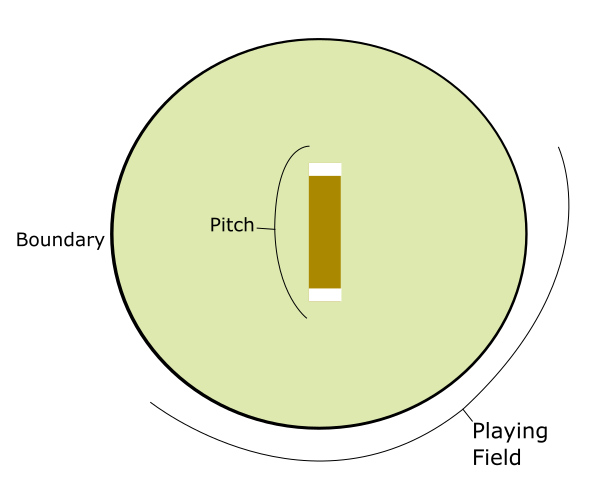
\includegraphics[width=0.7\linewidth]{figures/ptich.png}
    \caption{A basic cricket field}
\end{figure}

The game of cricket itself has two main forms. In this project we will only look at ``limited-overs cricket''. Cricket is played in ``overs'', each one consisting of 6 individual bowls delivered consecutively by the same bowler from one end of the pitch.
 Traditionally, there is no upper limit on the amount of overs a team may bowl, they keep going until the batting team ``declares'', meaning they believe they have a tactical advantage if they bowl now instead of later, or preferably for the bowling team, are all bowled out. 
Batters can be given ``out'' in quite a few different ways, but once a batter is out that is it, they don't get to bat again in that game. Once ten of the eleven players in the batting team have been given out, the innings comes to end and the team bowling 
gets their turn to bat. If they hit more runs before losing all of their ten wickets before the innings comes to an end, then they win. Cricket is an immensely complex game with countless intricacies and neuances, but at 
its core, applying mathematics to it is not an absurd proposition. \\

The traditional format of cricket, called ``first-class cricket'' lasts up to 4 days. This obviously has disadvantages from a spectator's point of view. 
In 1963, the cricketing calender in the UK had a different format of the game amended to it alongside the usual first-class fixtures.
The ``Gillette Cup'' introduced a form of cricket wherein each team only has 1 innings, lasting 50 overs instead of the prior method of no limit. The idea was 
that this competition, coming to a conclusion within the space of a day, would increase spectator numbers and by extension, ticket sales.  Rather than a league 
as is the structure with first class fixtures, this competition would be tournament based knock-out competition. This tournament ran for the last time in 2009, although 
a predecessor still populates the cricketing calender today. It is now known as the ``Royal London One-Day Cup'', however due to the introduction of other tournaments 
and so-called ``franchise cricket'' competitions, such as the Indian Premier League or Pakistan Super League,  the tournament has lost some relevancy in England and Wales. \\

Given the tournament-based nature of this new competition, we have the natural need for a definitive result.
This is something that is not always guaranteed in first class cricket, where draws are common.\footnote{Note that 
``draw'' and ``tie'' are not interchangeable terminology in cricket. A ``tie'' refers to achieving the exact same score, whereas a draw is where neither teams wins nor loses} As such, in order to allow for a result to be
determined when a game is cut short, the idea of target-revision was introduced. This meant that a team could be set a
roughly equivalent run target off of a reduced number of overs that would still classify them as the winners.
This is where Duckworth and Lewis came in, proposing their Duckworth-Lewis (DL) method \cite{duckworth}. As will be discussed in Chapter 3, the DL method 
has been slightly improved upon since it was published in the late 1990s, but the overarching philosophy of the method has stayed the same. 
One extension was that of Stern in 2004, \cite{stern}, now  known as the Duckworth-Lewis-Stern (DLS) method. This allowed for better score resetting in Twenty-20 (T20) cricket- an even shorter 
form of the game introduced to last only over the course of an afternoon instead of a day. 

\begin{example}
    Suppose a team bats first and score 340 in their 50 overs. The second team come out to chase and score 230 in 30 overs. At this point, it 
    starts to rain, and the umpire calls the players off the pitch. After half an hour the players go back out, but now there is only time for 10 overs 
    instead of the 20 that team 2 should have had. This is when the match officials would use the DLS method to set team 2 a reduced (but roughly equivalent) target, this may for example 
    lead to them needing 290 from 40 overs. 
\end{example}


\section{Problems with the Duckworth-Lewis-Stern Method}
$\cite{phanse}$ found that DLS has a bias towards not only the team batting first, but whoever won the coin toss at the start of the game.
They go onto to propose a simple extension to DLS for reducing these biases, but we won't cover that in this project. \\

DLS can also be prone to setting targets that are too extreme. We will see an example of this in Chapter 7. When such an absurd target is set, it 
can kill the game well before the end, since the batting team know that they cannot obtain the target, and are fighting an already lost battle. Not only 
is this bad for the batting team, but it ruins the game for spectators, some of whom may have paid considerable amounts of money and travelled far to spend the day watching the game. \\

\section{Project Aims}
The main aim of this project is to look at methods for \textit{predicting} cricket scores before resetting them. It is important to make the distinction between this 
and \textit{projecting} the scores, which is commonplace in the game at the minute. Projecting scores assumes a constant run rate, which it will be seen 
in later chapters is not really the case. However, we can make use of the patterns in run rates to try and extract a predictable score. At the lowest level,
we are going to train a neural network with inputs being run rates and an output being score. We can then pass the run rates of a game that gets cut short 
to this network, and it will try to predict a score based on the patterns in the runrates of that game.

The runrate is defined by the following formula, \\

\[
    \text{Run Rate}  = \frac{\text{Total Runs Scored}}{\text{Total Overs Bowled}}.
\]\\

This rate evolves as the game flows, and can skyrocket or plummet as one team or the other begins to outplay their opponent. To our knowledge, a run rate 
based neural network does not exist in the literature, and so our model is somewhat novel.

\section{Overview of Noteworthy Literature on Cricket Score Modelling}
We begin the look at literature on this topic with the paper published by F. Duckworth himself in 1998 \cite{duckworth}. In this paper, 
Duckworth proposes the ``D/L'' method. However, there is an issue with the sentence that appears after defining the function $Z(u,w)$;
``Comercial confidentiality prevents the disclosure of the mathematical definitions of these functions'', which means we can't access the actual parameters 
that they use for defining the model. This won't affect the development of our model, but it is unfortunate as it means getting a clear picture of DLS is slightly harder.
The claim is that these functions have been defined via experimentation, which gives rise to the first issue: the first T20 game of cricket was not played until 2003. 
So clearly, D/L was not designed with T20 in mind, and so the functions derived from experementation and research will not be accurate for T20 cricket. \\

In 2004, a year after the first T20 matches were played, Duckworth and Lewis published another paper \cite{duckworth2}, in which they report
that the table used for calculating the method can be employed by anyone at all levels of the game- from grass-roots cricket up to the highest standard of 
the professional game. The table is slightly updated as well due to the increased amount of data from which to calculate parameters. \\

Another noteworthy paper is that of \cite{saqlain}, looking at predicting scores from the 2019 Cricket World Cup, an ODI
tournament held across England. They used data after the previous world cup, held in Australia and New Zealand in 2015; all the way to $10^{th}$ November
2018. The interesting thing about this paper, is they do not use data from individual matches, but instead on 10 meta-statics, including 
``Number of series victories'', ``total wickets'', ``centuries'' and ``all out'', among others. They apply the TOPSIS method to this specific problem, using Algorithm~\ref{TOPSIS}. \\

\begin{algorithm}[h]
\caption{Modified TOPSIS Algorithm}\label{TOPSIS}
\begin{algorithmic}[1]
    \Require $m,n \geq 0$
    \State $\text{Calculate normalised matrix} \ X_{ij} = \frac{x_{ij}}{\sqrt{\sum_{i=1}^mx_{ij}^2}}$
    \State $\text{Calculate weighted normalised matrix} \ V_{ij}=X_{ij}W_j$
    \For{$i \in \{1,\ldots,m\}$}
        \State $\text{Calculate Euclidean distance from the best outcome } \ S_i^+ = \sqrt{\sum_{j=1}^n(V_{ij}-V_j^+)^2} \ $
        \State $\text{Calculate Euclidean distance from the worst outcome } \ S_i^- = \sqrt{\sum_{j=1}^n(V_{ij}-V_j^-)^2} \ $
    \EndFor
    \State $\text{Calculate performance score} \ C_i^* = \frac{S_i^-}{S_i^+  + S_i^-}$
\end{algorithmic}
\end{algorithm}

They used the results of this process to predict how the 2019 World Cup would look, rather than games for individual scores. However, they were largely unsuccessful. 
Not only did the authors leave Sri Lanka out of their calculations entirely, they only successfully predicted India would finish top of the points table, and Afghanistan 
at the bottom. It's worth mentioning that this may not be an issue with the mathematical model itself, but the imbalance of data. Teams like Afghanistan play far fewer games 
than a team like England or India. This introduces a bias favouring teams who have played more games not only from a statistical point of view, but from a cricketing one too 
since the teams that play less will have less match practice going into a big tournament like the World Cup. \\

However, the paper \cite{kumar} takes an approach along the same lines of the aim of this project. It is not necessary to discuss the individual aspects
of their paper here, as it will be discussed in Chapter 5, when we build our model. However it is worth noting the results of this paper now to see how
ours differ. They found their limited dataset to be a problem in classifying. This is something we have been aware of, but there isn't much that can be done
given the nature of how many cricket games are played per year. This limiting factor is certainly not trivial, but means returning to this study in future 
will more than likely lead to more accurate and refined predictions. \\

Machine learning is certainly not new to cricket, \cite{kampakis} managed to predict the winners in English T20 cricket in ``almost two thirds'' of their test cases. While this 
is a fantastic result, in this dissertation we have not concerned ourselves with directly predicting winners, but actual scores. This is again something that is hard to find 
in cricket specific literature, so we have taken inspiration from industries such as finance, as well as other sports in building our model. 